% !TeX program = xelatex
\RequirePackage{fix-cm}
\documentclass[14pt,a4paper]{extarticle}
\usepackage{fontspec}
\defaultfontfeatures{Ligatures=TeX}
\input{build/font-path.tex}
\ifdefined\reportFontPath
  \setmainfont{Times.TTF}[Path=\reportFontPath,BoldFont=Timesbd.TTF,ItalicFont=Timesi.TTF,BoldItalicFont=Timesbi.TTF]
  \newfontfamily\cyrillicfont{Times.TTF}[Path=\reportFontPath,BoldFont=Timesbd.TTF,ItalicFont=Timesi.TTF,BoldItalicFont=Timesbi.TTF,Script=Default]
\else
  \setmainfont{Times New Roman}
  \newfontfamily\cyrillicfont{Times New Roman}
\fi
\setmonofont{FreeMono}
\newfontfamily\cyrillicfonttt{FreeMono}
\usepackage{polyglossia}
\setdefaultlanguage{russian}
\setotherlanguage{english}
\usepackage[left=30mm,right=10mm,top=20mm,bottom=20mm,footskip=10mm]{geometry}
\usepackage{setspace}
\makeatletter
\renewcommand{\normalsize}{\@setfontsize\normalsize{14bp}{16.8bp}}
\makeatother
\onehalfspacing
\AtBeginDocument{\normalsize}
\setlength{\parindent}{1.25cm}
\setlength{\parskip}{0pt}
\usepackage{indentfirst}
\usepackage{array,tabularx,graphicx,float,caption,fancyvrb}
\DeclareCaptionLabelSeparator{gost}{~—~}
\captionsetup{font=small,labelsep=gost,justification=centering,singlelinecheck=false}
\captionsetup[table]{justification=raggedright,position=top,skip=6pt}
\captionsetup[figure]{skip=8pt}
\addto\captionsrussian{\renewcommand{\figurename}{Рисунок}\renewcommand{\tablename}{Таблица}}
\usepackage{titlesec}
\titleformat{\section}[block]{\normalfont\bfseries\centering}{\thesection.}{.5em}{\MakeUppercase}
\titlespacing*{\section}{0pt}{0pt}{18pt}
\usepackage{enumitem}
\usepackage{xurl}
\urlstyle{same}
\usepackage[hidelinks,unicode,pdfauthor={Матвеев М. А.},pdftitle={Лабораторная работа №1. Оформление и стилизация текста}]{hyperref}
\pagestyle{plain}
\emergencystretch=2em
\clubpenalty=10000
\widowpenalty=10000
\raggedbottom
\newcolumntype{Y}{>{\raggedright\arraybackslash}X}
\newcommand{\code}[1]{{\fontsize{12}{14}\selectfont\texttt{#1}}}
\newcommand{\listing}[1]{\begingroup\singlespacing\VerbatimInput[fontsize=\fontsize{10}{12.5}\selectfont,numbers=left,numbersep=6pt,xleftmargin=16pt]{#1}\endgroup}

\begin{document}
\begin{titlepage}
\thispagestyle{empty}
\begin{center}
\bfseries
МИНОБРНАУКИ РОССИИ\\
Федеральное государственное автономное\\
образовательное учреждение высшего образования\\
«Санкт-Петербургский государственный\\
электротехнический университет «ЛЭТИ»\\
им. В.И. Ульянова (Ленина)»\\
Кафедра информационных систем
\end{center}
\vspace{30mm}
\begin{center}
\textbf{ОТЧЕТ ПО ЛАБОРАТОРНОЙ РАБОТЕ №1}\\[8mm]
«Оформление и стилизация текста»
\end{center}
\vfill
\noindent\begin{tabularx}{\textwidth}{@{}lXr@{}}
Студент гр. 4372 & \centering\rule{25mm}{0.3pt} & Матвеев М. А.\\[8mm]
Преподаватель & \centering\rule{25mm}{0.3pt} & Нечитайленко Р. А.\\
\end{tabularx}
\vspace{20mm}
\begin{center}
Санкт-Петербург\\
2026
\end{center}
\end{titlepage}
\setcounter{page}{2}

\section{Цель и выполнение работы}
Цель работы: создать HTML-страницу и оформить текст с помощью внешней таблицы стилей CSS.

В каталоге \code{lab-01} размещены \code{index.html} и \code{style.css}. Страница содержит заголовок первого уровня, два абзаца, заголовок второго уровня и маркированный список из трёх пунктов. CSS подключён элементом \code{link} в разделе \code{head}.

Первое правило CSS относится к \code{body}. Оно задаёт семейство шрифтов Arial, sans-serif, размер 16~px, цвет \code{\#333} и межстрочный интервал 1,5. Отдельные элементы оформлены классами \code{title}, \code{subtitle} и \code{list} (таблица~\ref{tab:styles}).

\begin{table}[H]
\caption{Стили элементов страницы}\label{tab:styles}
\begingroup\fontsize{12}{14}\selectfont\singlespacing
\renewcommand{\arraystretch}{1.25}
\begin{tabularx}{\textwidth}{|l|l|l|Y|}
\hline
Класс & Размер & Цвет & Оформление\\ \hline
\code{title} & 40 px & \code{\#f03333} & Прописные буквы, интервал 1,2\\ \hline
\code{subtitle} & 30 px & \code{\#12ac11} & Подчёркивание, интервал 1,2\\ \hline
\code{list} & 20 px & \code{\#444} & Курсив, квадратные маркеры\\ \hline
\end{tabularx}
\endgroup
\end{table}

\begin{figure}[H]
\centering
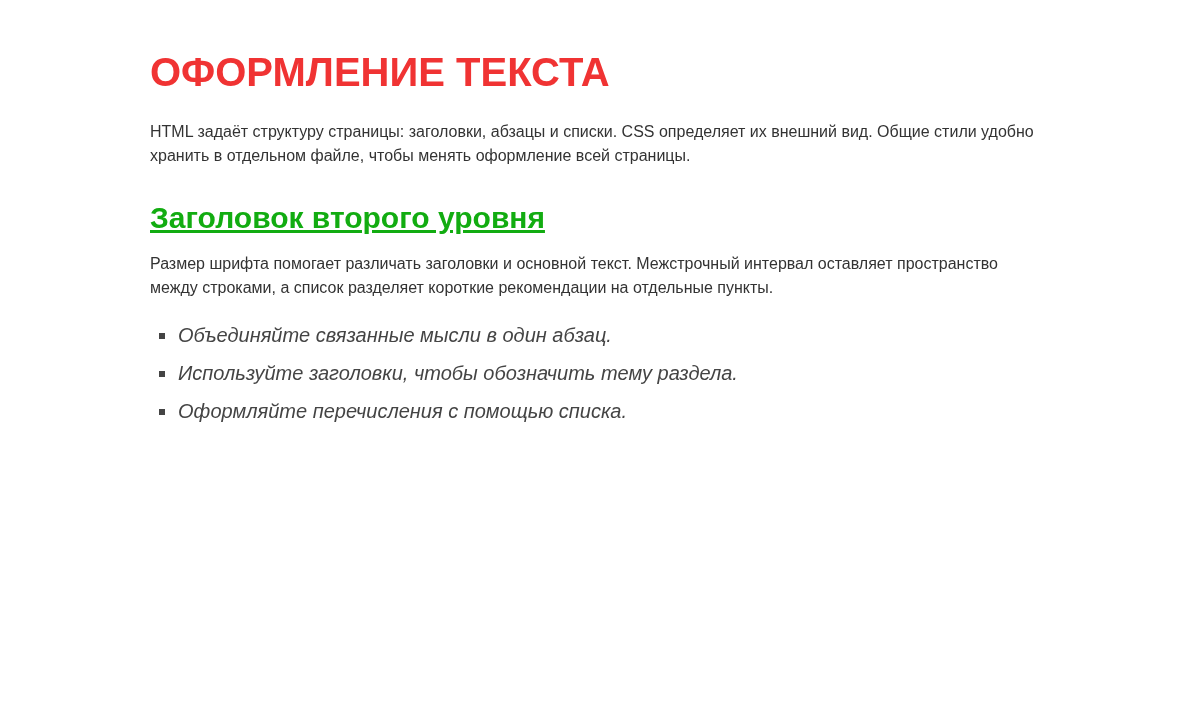
\includegraphics[width=\textwidth]{assets/desktop.png}
\caption{Страница при ширине окна 1200 px}\label{fig:desktop}
\end{figure}

\clearpage
\section{HTML-разметка}
Документ использует кодировку UTF-8 и атрибут \code{lang="ru"}. Метатег \code{viewport} задаёт ширину области просмотра по ширине устройства. Текст списка размещён в элементах \code{li}, вложенных в \code{ul}.

\vspace{4mm}
\noindent Исходный код \code{index.html}:
\listing{../index.html}

\clearpage
\section{Таблица стилей}
Ширина текстовой области ограничена 900~px. Внешние отступы центрируют её, внутренние отступы отделяют текст от краёв окна. Свойство \code{overflow-wrap: anywhere} разрешает перенос длинного слова в главном заголовке на узком экране.

\vspace{4mm}
\noindent Исходный код \code{style.css}:
\listing{../style.css}

\clearpage
\section{Проверка результата}
Страница проверена в Chromium 153.0.8010.52. Вычисленные браузером стили совпали с заданными значениями: основной текст имеет размер 16~px и высоту строки 24~px, заголовки имеют размеры 40 и 30~px и высоту строки 48 и 36~px соответственно. Список содержит ровно три пункта с квадратными маркерами и курсивом.

При ширине окна 1440, 1200, 375 и 320~px горизонтальная прокрутка отсутствует. На узком экране заголовки и абзацы переносятся на следующие строки. Файл стилей загружается успешно, ошибок JavaScript при открытии страницы не зафиксировано.

\begin{figure}[H]
\centering
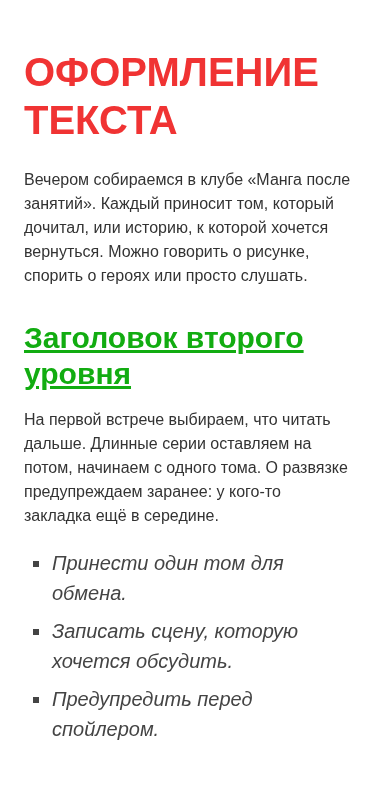
\includegraphics[height=150mm]{assets/mobile.png}
\caption{Страница при ширине окна 375 px}\label{fig:mobile}
\end{figure}

\clearpage
\section*{Заключение}
Создана страница с заголовками двух уровней, абзацами и маркированным списком. Оформление вынесено в отдельный CSS-файл. При проверке подтверждены заданные размеры, цвета, межстрочные интервалы и оформление элементов. Страница сохраняет читаемость на узком экране.


\clearpage
\section*{Список использованных источников}
\begin{enumerate}[label=\arabic*.,leftmargin=8mm,itemsep=8pt,parsep=0pt]
\item text-transform // HTMLbook.ru. URL: \url{https://htmlbook.ru/css/text-transform} (дата обращения: 20.10.2026).
\item text-decoration // HTMLbook.ru. URL: \url{https://htmlbook.ru/css/text-decoration} (дата обращения: 20.10.2026).
\item list-style-type // HTMLbook.ru. URL: \url{https://htmlbook.ru/css/list-style-type} (дата обращения: 20.10.2026).
\item line-height // HTMLbook.ru. URL: \url{https://htmlbook.ru/css/line-height} (дата обращения: 20.10.2026).
\end{enumerate}
\end{document}
